%%%%%%%%%%%%%%%%%%%%%%%%%%%%%%%%%%%%%%%%%%%%%%%%%%%%%%%%%%%%%%%%%%%%%%%%%%%

\documentclass[a4paper,oneside,12pt]{article}
\usepackage{mystyle}

\begin{document}

\title{\Large\bf Approximation}
\author{%%
  Minh Van Nguyen \\
  \url{mvngu@gmx.com}
}
\date{\today}
\maketitle

%%%%%%%%%%%%%%%%%%%%%%%%%%%%%%%%%%%%%%%%%%%%%%%%%%%%%%%%%%%%%%%%%%%%%%%%%%%

\section{The number $\pi$}

The number $\pi = 3.141592\dots$ is another example of an irrational
number.  The number $\pi$ is often used to measure the area and
circumference of a circle; see \Figure{fig:general_circle}.  Since
$\pi$ is irrational, the number cannot be written as a ratio of
integers.  So for practical purposes, you must approximate $\pi$ as
closely as you can.  The Greek mathematician Archimedes used the
fraction $22 / 7$ to approximate $\pi$.  The fraction $22 / 7$ can be
written as $22 / 7 = 3.142857$, correct to six decimal digits.  This
is not a good approximation to $\pi$ because the value of $22 / 7$
differs from $\pi$ from the third decimal digit onwards.  If a number
$p \in \RR$ is to be a good approximation of $\pi$, then it should be
possible to make $p$ as close to $\pi$ as you want.

\begin{figure}[!htbp]
\centering
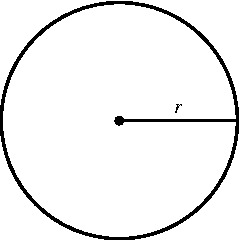
\includegraphics[scale=1]{image/03/circle.pdf}
\caption{%%
  A circle with radius $r$.  Since the radius cannot be negative or
  zero, you must have $r > 0$.  The \emph{radius} of a circle is
  defined as the distance from the centre of the circle to any point
  on the circle.  The \emph{diameter}, denoted $d$, is then defined as
  twice the radius, i.e.~$d = 2r$.  The distance around the circle is
  called its \emph{circumference}.
}
\label{fig:general_circle}
\end{figure}

In order to approximate $\pi$ as closely as possible, you must know
how $\pi$ is defined.  Let $c$ be the circumference of a circle and
let $d$ be the diameter of the same circle.  Then the value of $\pi$
is defined as the ratio
%%
\begin{equation}
\label{eqn:define_pi_as_ratio_of_c_over_d}
\pi
=
\frac{c}{d}.
\end{equation}
%%
But now you have two problems:
%%
\begin{packedenumeral}
\item How is the value of the diameter $d$ determined?

\item How do you calculate the value of the circumference $c$?
\end{packedenumeral}
%%
The short answer is: You approximate the values of $d$ and $c$ and
then substitute those values into
\Equation{eqn:define_pi_as_ratio_of_c_over_d} to obtain an
approximation of $\pi$.  What follows is the long answer.


%%%%%%%%%%%%%%%%%%%%%%%%%%%%%%%%%%%%%%%%%%%%%%%%%%%%%%%%%%%%%%%%%%%%%%%%%%%

\section{Coordinates}


%%%%%%%%%%%%%%%%%%%%%%%%%%%%%%%%%%%%%%%%%%%%%%%%%%%%%%%%%%%%%%%%%%%%%%%%%%%

\section{Approximating $\pi$ with a square}

Let's start by approximating the value of $\pi$ with a square.  The
square is drawn inside a unit circle such that the four corners of the
square touch the circle; see \Figure{fig:circle_inscribed_square}.

\begin{figure}[!htbp]
\centering
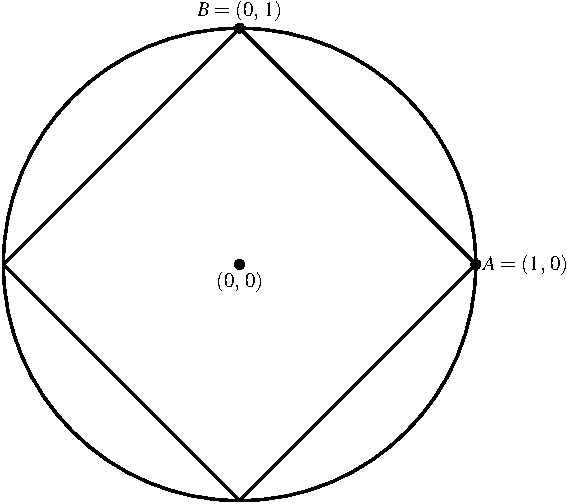
\includegraphics[scale=1]{image/03/circle-square.pdf}
\caption{%%
  A unit circle with an inscribed square.  A \emph{unit circle} is a
  circle whose radius is $1$.  The centre of the circle has
  coordinates $\tuple{0}{0}$.  The points $A$ and $B$ are where the
  square touches the circle.
}
\label{fig:circle_inscribed_square}
\end{figure}

\end{document}
